\section{Model deployment}
\subsection{Deploy the model locally using Voila}

Voilà allows you to convert a Jupyter Notebook into an interactive dashboard that allows you to share your work with others. It is secure and customizable, giving you control over what your readers experience \cite{Voila}.

Install Voila with conda (figure \ref{figure:Voila}).

\begin{figure}[H]
	\centering
	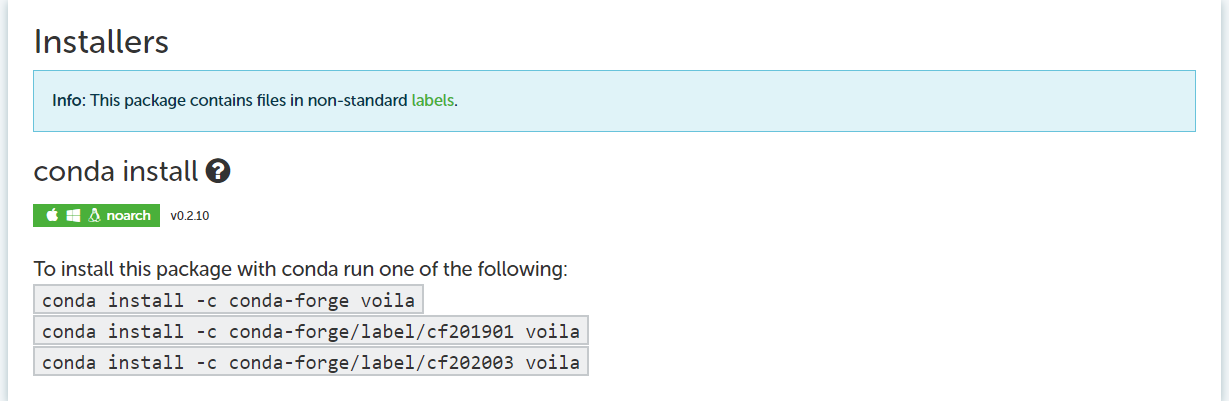
\includegraphics[width=0.8\columnwidth]{Pictures/Voila.png}
	\caption[Short title]{Voila package install}
	\label{figure:Voila}
\end{figure}

Move to the Jupiter notebook directory using cd "name of directory" and Run the Voila command : voila \textcolor{	red}{notebooknames}.ipynb. An example is shown in figure \ref{figure:Voila Run}.

\begin{figure}[H]
	\centering
	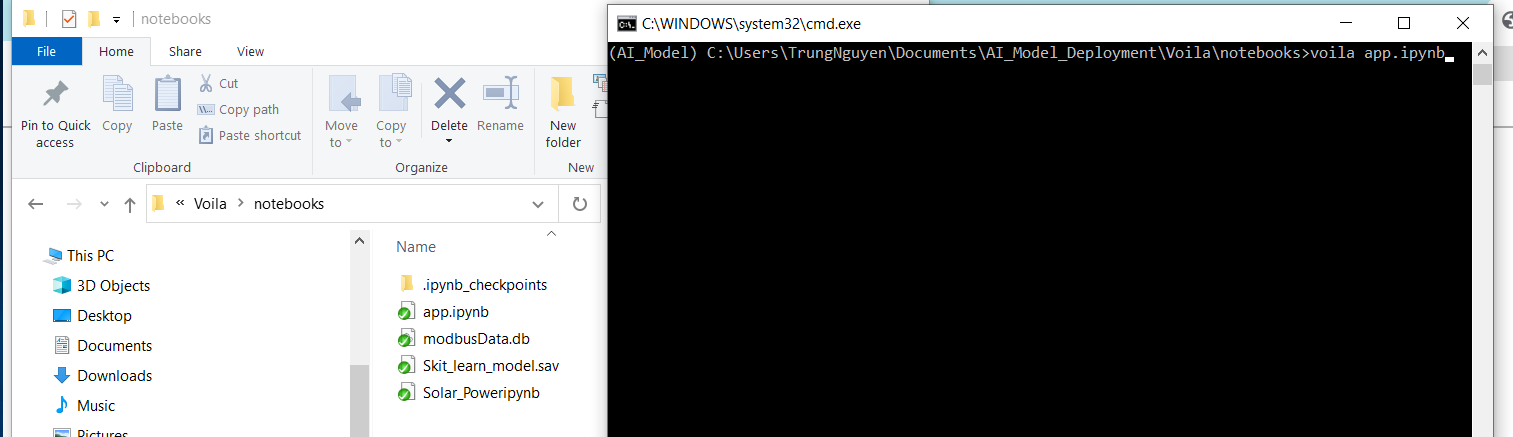
\includegraphics[width=0.8\columnwidth]{Pictures/Voila Run command.png}
	\caption[Short title]{Voila Run Command}
	\label{figure:Voila Run}
\end{figure}

A web browser with localhost address (figure \ref{figure:Voila Web}) will be 
opened 

\begin{figure}[H]
	\centering
    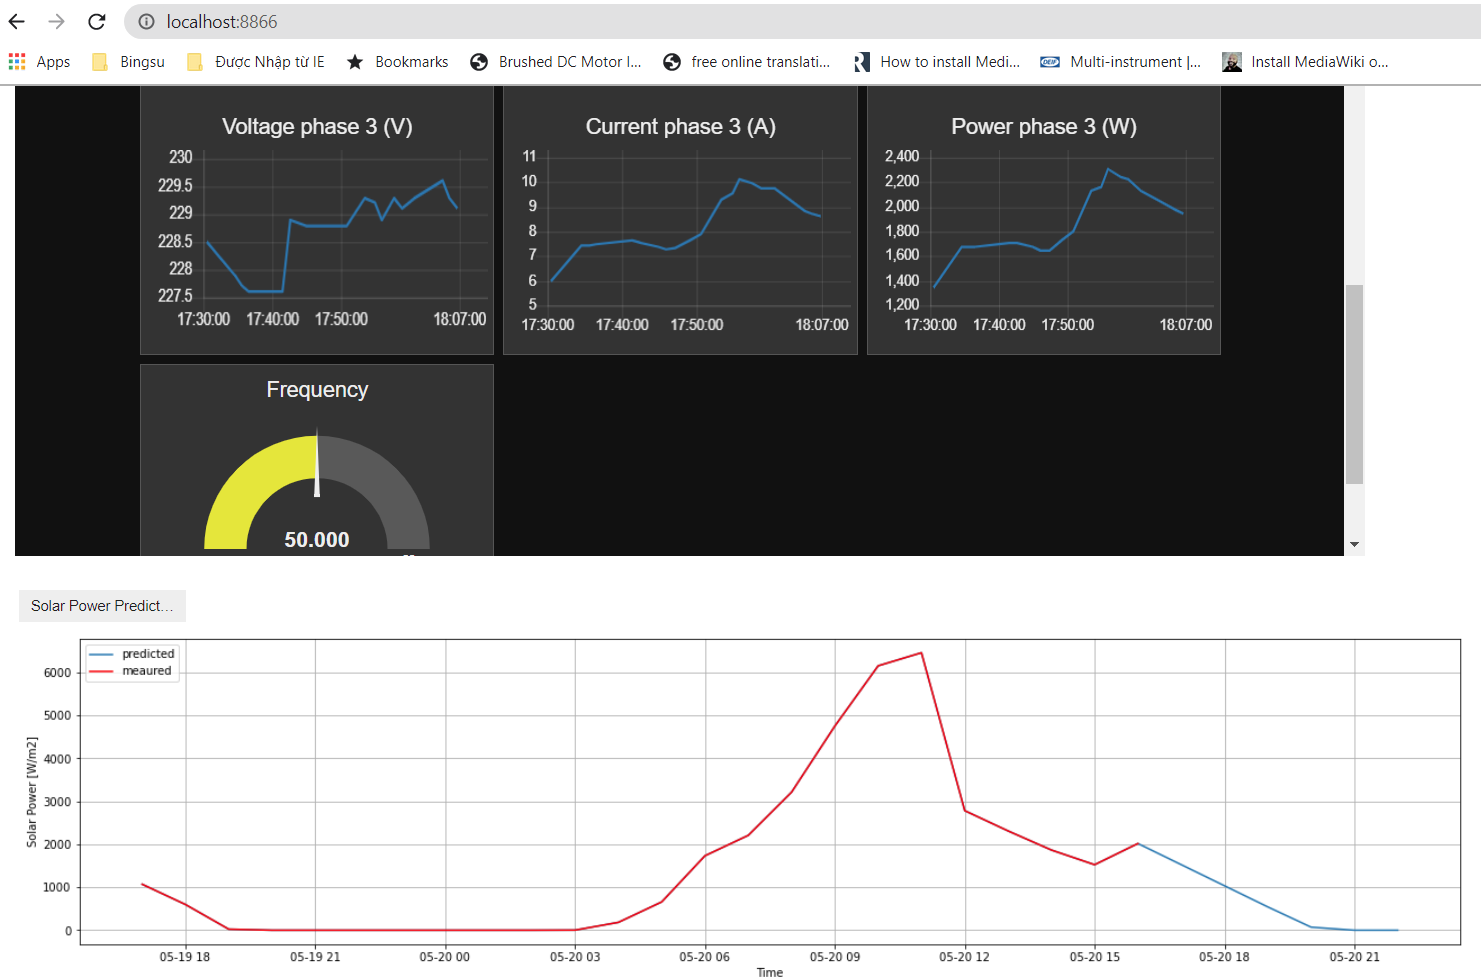
\includegraphics[width=0.8\columnwidth]{Pictures/Voila web example.png}
	\caption[Short title]{Voila Web}
	\label{figure:Voila Web}
\end{figure}

% https://voila.readthedocs.io/en/stable/deploy.html

\subsection{Deploy the model with Heroku}

Heroku is a cloud Platform that helps developers quickly deploy, manage, and scale moderns applications. Heroku provide a free package for non commercial app such as proof of concept and personal project \ref{figure:Heroku pricing}.

\begin{figure}[H]
	\centering
    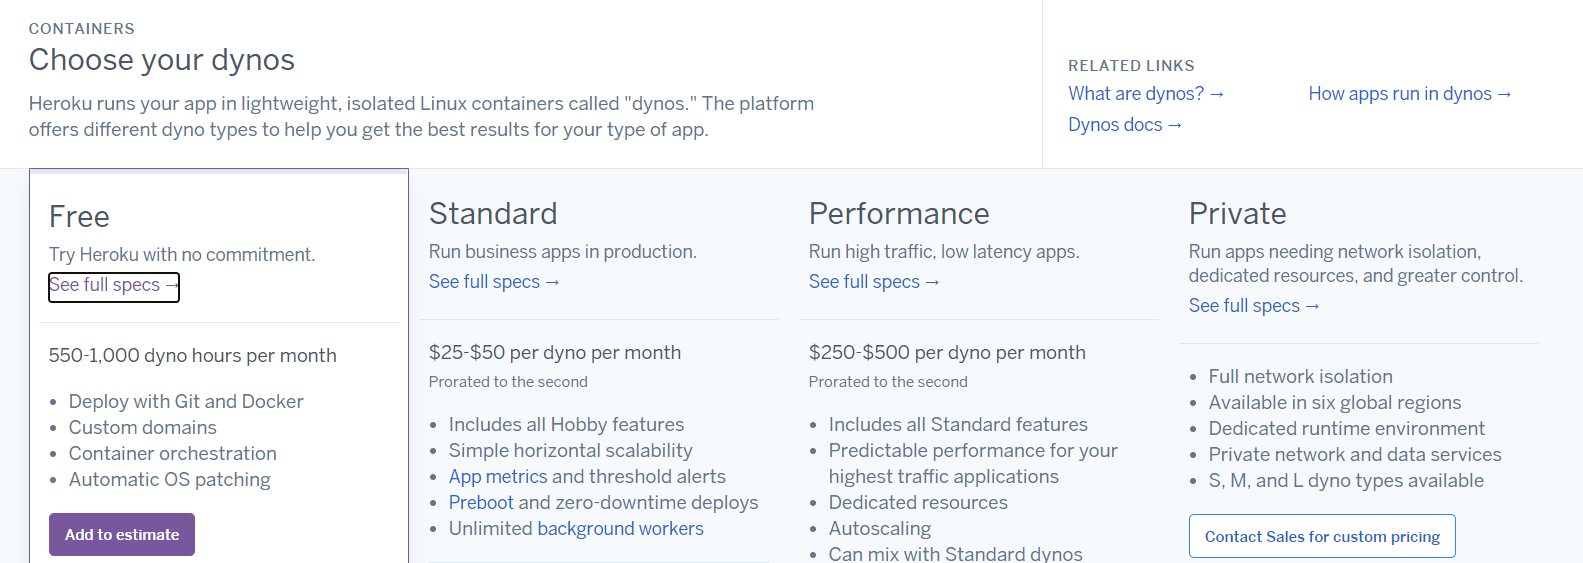
\includegraphics[width=0.8\columnwidth]{Pictures/Heroku packages.png}
	\caption[Short title]{Heroku Pricing}
	\label{figure:Heroku pricing}
\end{figure}

The first step is to create three files that Heroku requires.

\begin{itemize}
    \item requirements.txt : tells Heroku which Python packages to install when it run the web app.
    \item runtime.txt : specifies the version of Python we want Heroku to use.
    \item procfile: This file includes the instructions for Heroku to deploy our Voila app.
\end{itemize}

An example github prepare for Heroku deployment is shown on figure \ref{figure:Heroku github}. The notebooks folder content the jupyternotebook. 

\begin{figure}[H]
	\centering
    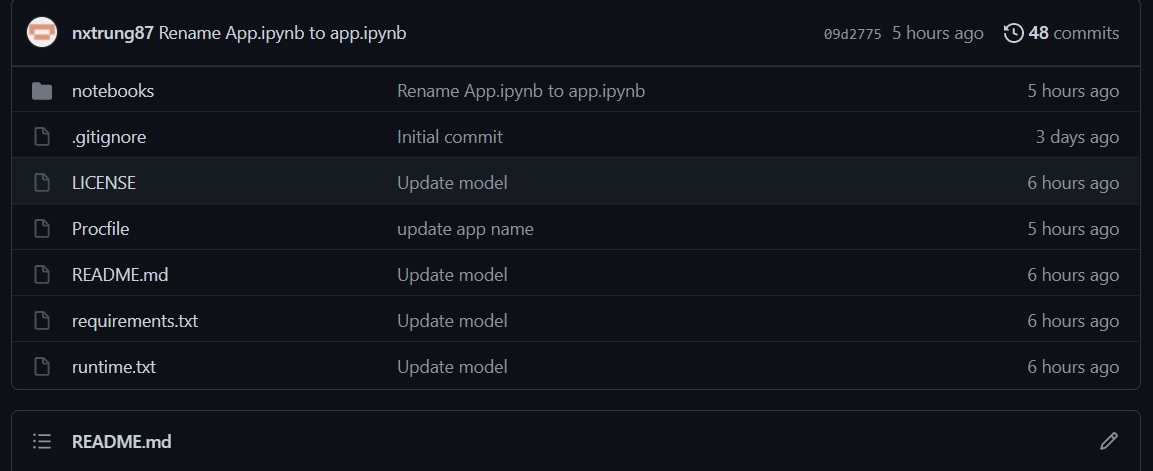
\includegraphics[width=0.8\columnwidth]{Pictures/Hroku_git.jpg}
	\caption[Short title]{Heroku github example}
	\label{figure:Heroku github}
\end{figure}

The contents example of the three Heroku require files is shown on figure \ref{figure:Heroku file content}. On the top left of the figure is the requirements.txt, top right is the runtuime.txt and bottom is the Procfile.

\begin{figure}[H]
	\centering
    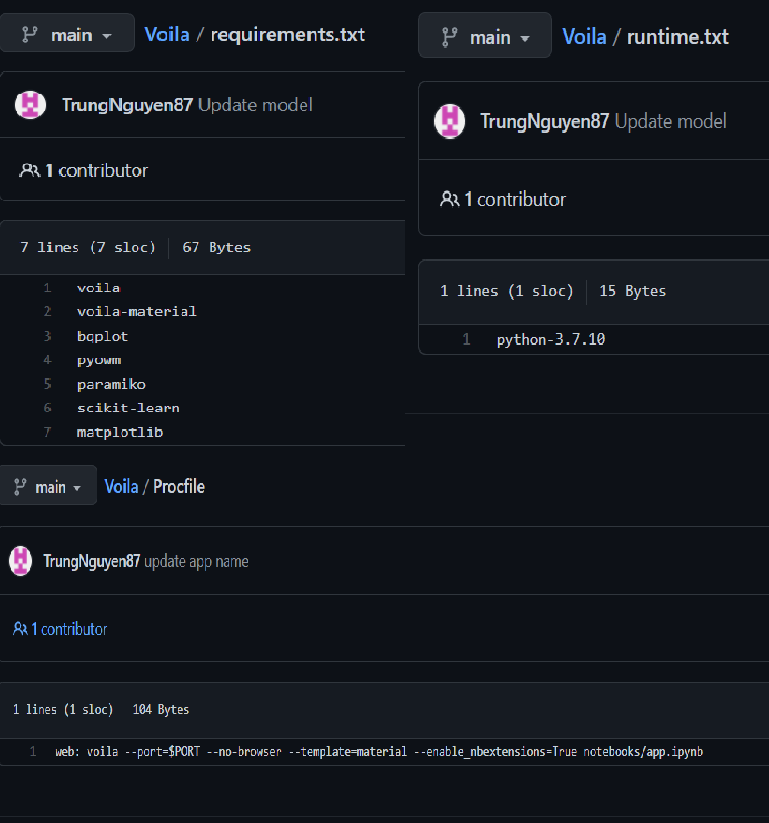
\includegraphics[width=0.8\columnwidth]{Pictures/Voila_heroku_files.png}
	\caption[Short title]{Heroku files content example}
	\label{figure:Heroku file content}
\end{figure}

\newpage

Next step is create an account with Heroku and follow the instruction in figure \ref{figure:Create new app}, \ref{figure:Create new app ctn}, \ref{figure:setup deployment}, \ref{figure:setup deployment method}, \ref{figure:web link}

In figure \ref{figure:Create new app} select new on the right corner.

\begin{figure}[H]
	\centering
    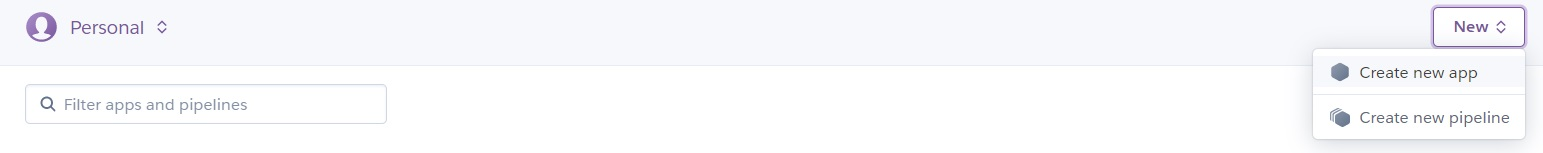
\includegraphics[width=0.8\columnwidth]{Pictures/Heroku_newapp.jpg}
	\caption[Short title]{Create new app}
	\label{figure:Create new app}
\end{figure}

Give a name for the app using lower letter case, select the deployment region and then select the create app button on the bottom.

\begin{figure}[H]
	\centering
    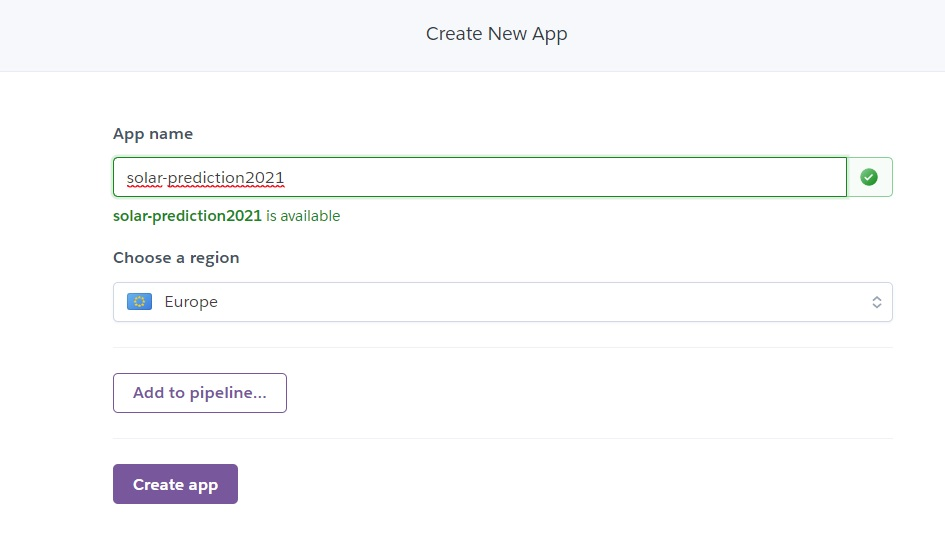
\includegraphics[width=0.8\columnwidth]{Pictures/Heroku_app.jpg}
	\caption[Short title]{Create new app ctn}
	\label{figure:Create new app ctn}
\end{figure}

In figure \ref{figure:setup deployment} select the Deploy tab and connect your app github repository. Scroll down and choose to enable the automatic deploys in figure \ref{figure:setup deployment method}.

Automatic deploys means every time when something is changed (for example update the requirement file or code file), the web app will also be updated. 

\begin{figure}[H]
	\centering
    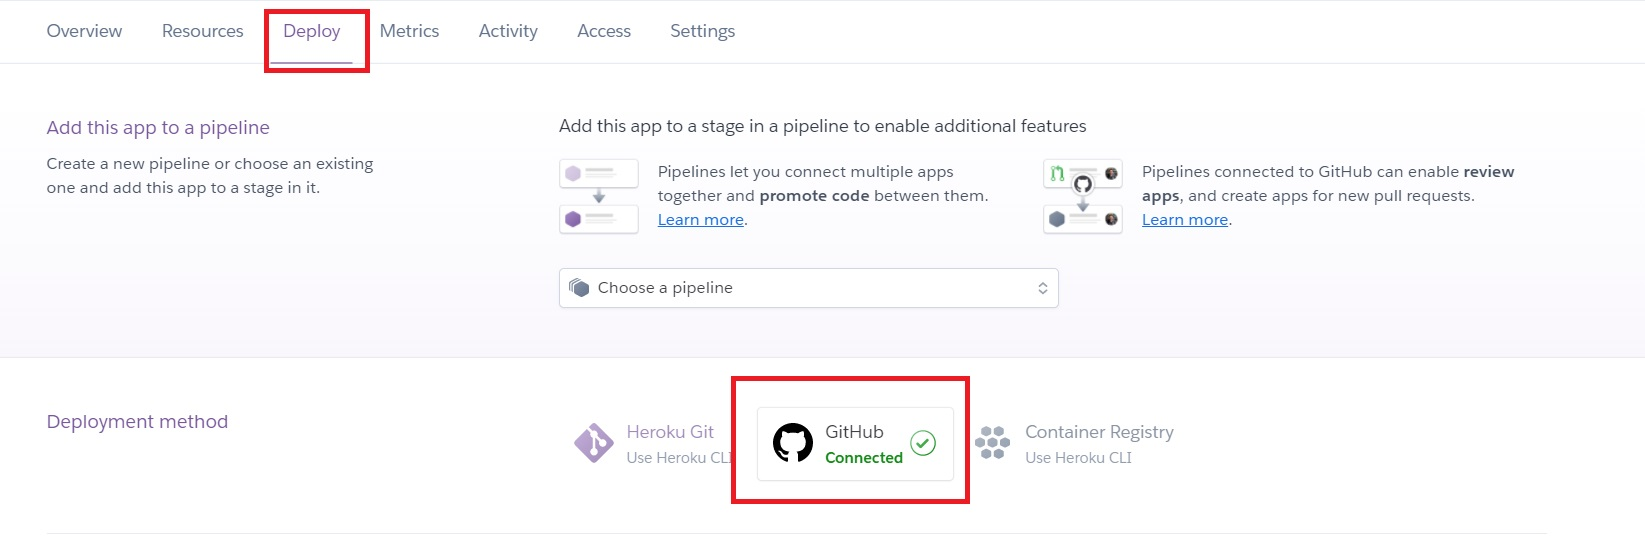
\includegraphics[width=0.8\columnwidth]{Pictures/Heroku_Deployment_setting.jpg}
	\caption[Short title]{Set up deployment}
	\label{figure:setup deployment}
\end{figure}

\begin{figure}[H]
	\centering
    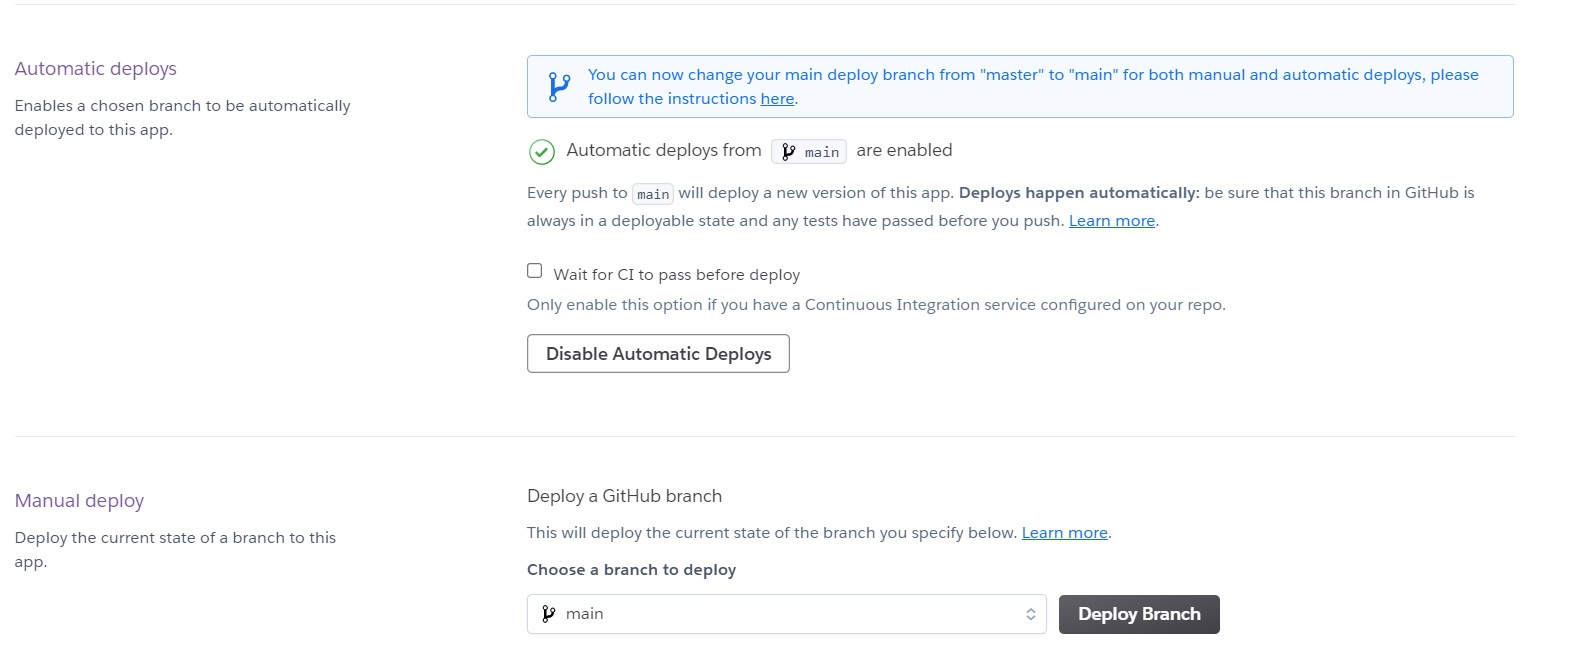
\includegraphics[width=0.8\columnwidth]{Pictures/Heroku_Deployment_methods.jpg}
	\caption[Short title]{Set up deployment method}
	\label{figure:setup deployment method}
\end{figure}

Link to the web app can be found on setting tab, scroll down to domains section (figure \ref{figure:web link}). User can also add their own domain name.

\begin{figure}[H]
	\centering
    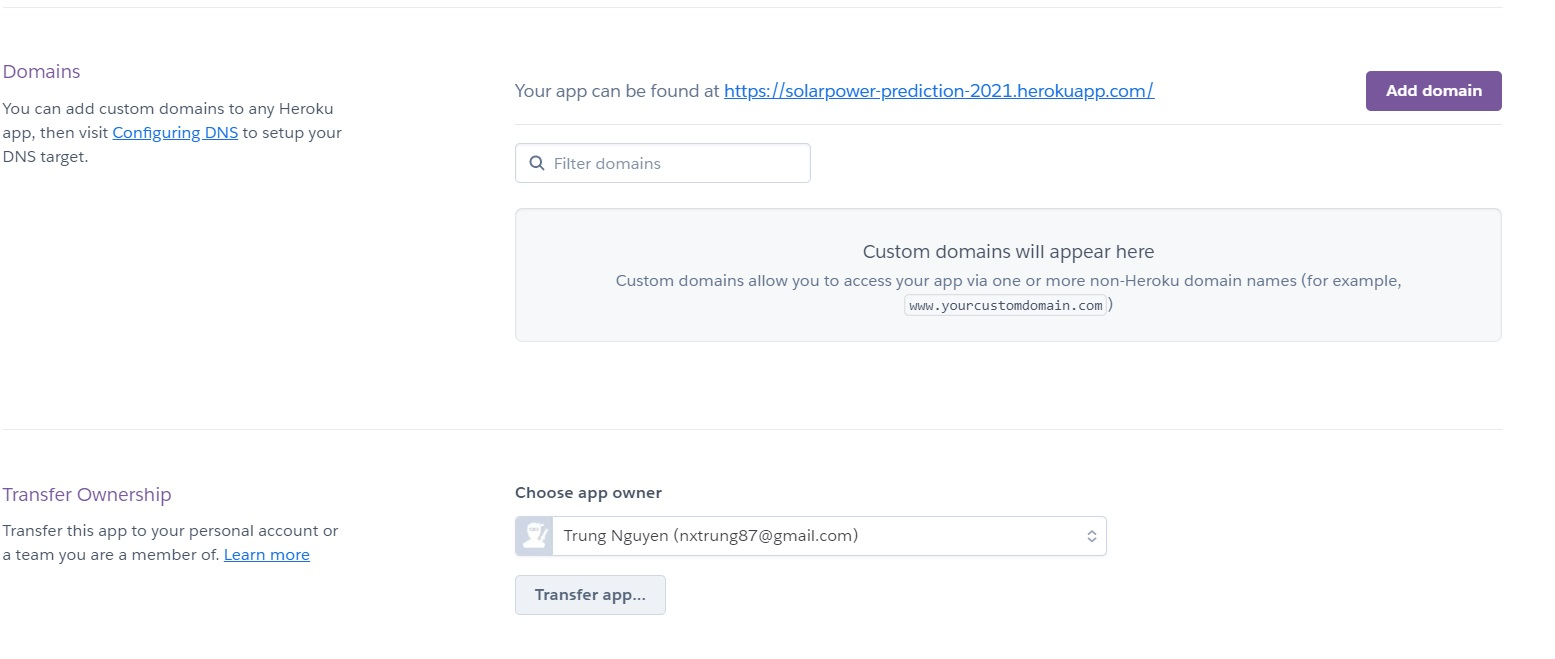
\includegraphics[width=0.8\columnwidth]{Pictures/Personal webapp.jpg}
	\caption[Short title]{Link of the web app}
	\label{figure:web link}
\end{figure}

Figure \ref{figure:web app} is a demo web app.

\begin{figure}[H]
	\centering
    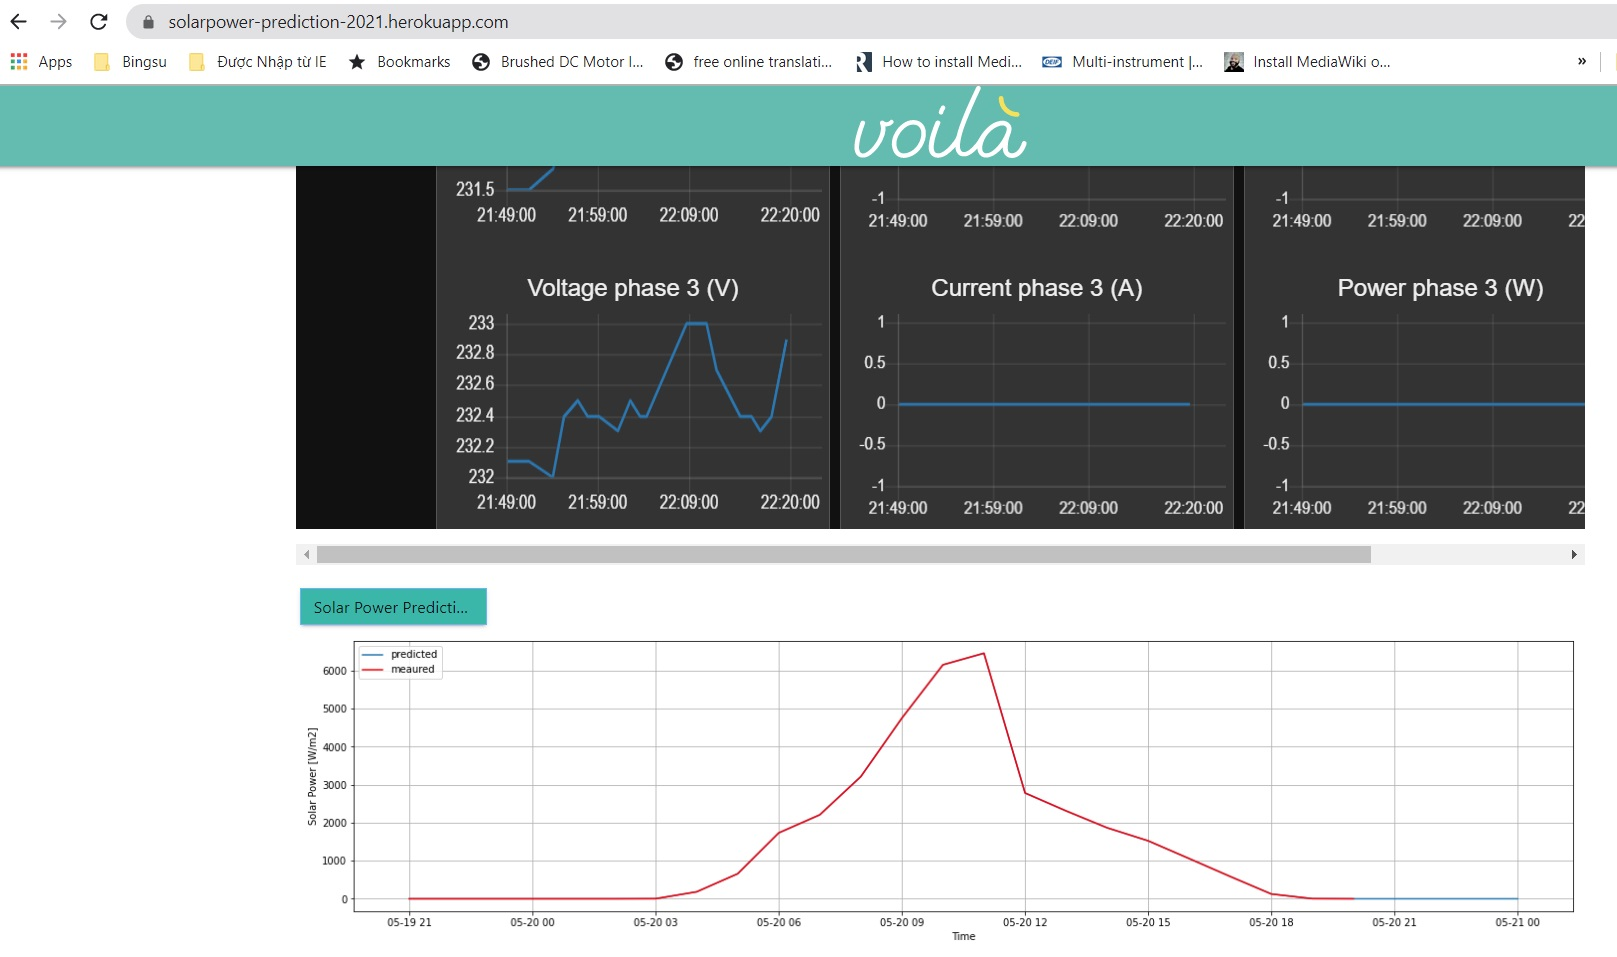
\includegraphics[width=0.8\columnwidth]{Pictures/Demo webapp.jpg}
	\caption[Short title]{The demo webapp}
	\label{figure:web app}
\end{figure}

\subsection{Forked the demo Github}

For the users who would like to try something quick. Forked the demo github repository (figure \ref{figure:Forked repo}) using the forked button on top right of the demo github page and follow the instruction to setup the deployment app with Heroku in the previous section.

\begin{figure}[H]
	\centering
    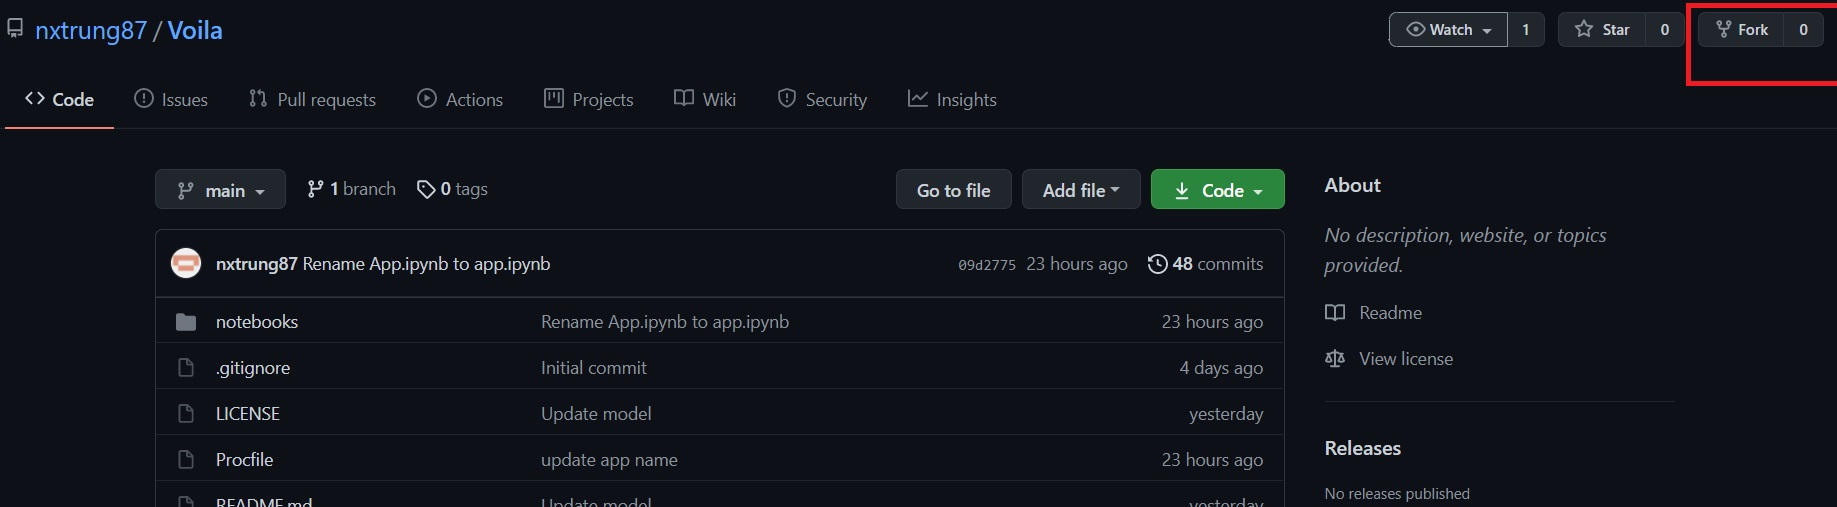
\includegraphics[width=0.8\columnwidth]{Pictures/forked repository.jpg}
	\caption[Short title]{Forked a repository}
	\label{figure:Forked repo}
\end{figure}

A few more demo github page to try out:
\begin{itemize}
    \item \hyperlink{https://github.com/voila-dashboards/voila-heroku}{voila-heroku}.
    \item \hyperlink{https://github.com/maartenbreddels/voila-demo}{voila-demo}.
    \item \hyperlink{https://github.com/jtpio/jupyterlab-heroku}{jupyterlab-heroku}.
\end{itemize}


\newpage
